

\documentclass{article}
\usepackage[utf8]{inputenc}
\usepackage[utf8]{inputenc}
\usepackage[T1]{fontenc}
\usepackage[english]{babel}
\usepackage{fullpage}
\usepackage{color}
\usepackage[table]{xcolor}
\usepackage{listings}
 
\definecolor{darkWhite}{rgb}{0.94,0.94,0.94}
 
\lstset{
  aboveskip=3mm,
  belowskip=-2mm,
  backgroundcolor=\color{darkWhite},
  basicstyle=\footnotesize,
  breakatwhitespace=false,
  breaklines=true,
  captionpos=b,
  commentstyle=\color{red},
  deletekeywords={...},
  escapeinside={\%*}{*)},
  extendedchars=true,
  framexleftmargin=16pt,
  framextopmargin=3pt,
  framexbottommargin=6pt,
  frame=tb,
  keepspaces=true,
  keywordstyle=\color{blue},
  language=C,
  literate=
  {²}{{\textsuperscript{2}}}1
  {⁴}{{\textsuperscript{4}}}1
  {⁶}{{\textsuperscript{6}}}1
  {⁸}{{\textsuperscript{8}}}1
  {€}{{\euro{}}}1
  {é}{{\'e}}1
  {è}{{\`{e}}}1
  {ê}{{\^{e}}}1
  {ë}{{\¨{e}}}1
  {É}{{\'{E}}}1
  {Ê}{{\^{E}}}1
  {û}{{\^{u}}}1
  {ù}{{\`{u}}}1
  {â}{{\^{a}}}1
  {à}{{\`{a}}}1
  {á}{{\'{a}}}1
  {ã}{{\~{a}}}1
  {Á}{{\'{A}}}1
  {Â}{{\^{A}}}1
  {Ã}{{\~{A}}}1
  {ç}{{\c{c}}}1
  {Ç}{{\c{C}}}1
  {õ}{{\~{o}}}1
  {ó}{{\'{o}}}1
  {ô}{{\^{o}}}1
  {Õ}{{\~{O}}}1
  {Ó}{{\'{O}}}1
  {Ô}{{\^{O}}}1
  {î}{{\^{i}}}1
  {Î}{{\^{I}}}1
  {í}{{\'{i}}}1
  {Í}{{\~{Í}}}1,
  morekeywords={*,...},
  numbers=left,
  numbersep=10pt,
  numberstyle=\tiny\color{black},
  rulecolor=\color{black},
  showspaces=false,
  showstringspaces=false,
  showtabs=false,
  stepnumber=1,
  stringstyle=\color{gray},
  tabsize=4,
  title=\lstname,
}
\usepackage{graphicx}
\graphicspath{ {./images/} }
\title{HAI804I – Analyse et Traitement d'Images}
\author{Fabien Caballero }

\begin{document}

\maketitle
    \tableofcontents

\newpage

\begin{figure}[h]
\centerline{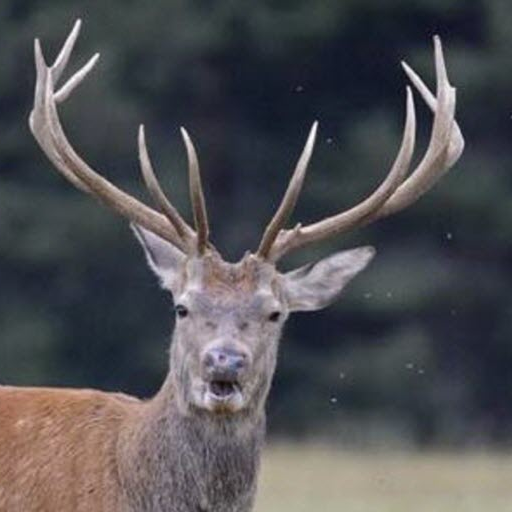
\includegraphics[scale=0.4]{./rendus/cerf.png}  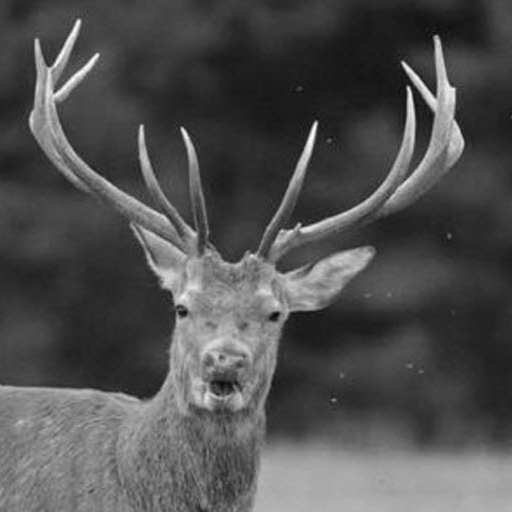
\includegraphics[scale=0.4]{./rendus/cerfgris.png}}
\caption{Image d'origine utilisée le long du TP}
\end{figure}

\section{Seuillage d'une image au format pgm}


\begin{figure}[h]
\centerline{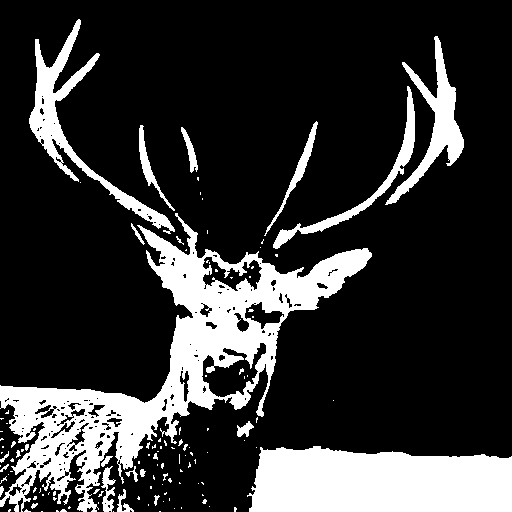
\includegraphics[scale=0.3]{./rendus/cerf1Seuil.png}}
\caption{cerf.pgm avec un seuil de 128}
\end{figure}

Pour le seuillage, on parcours chaque pixel et on teste sa valeur si celle-ci est inférieure au seuil on met à 0 (noir) ce pixel dans le tableau de l'image de sortie, sinon à 255 (blanc).

\section{Seuillage d'une image au format pgm avec 3 seuils }

\begin{figure}[h]
\centerline{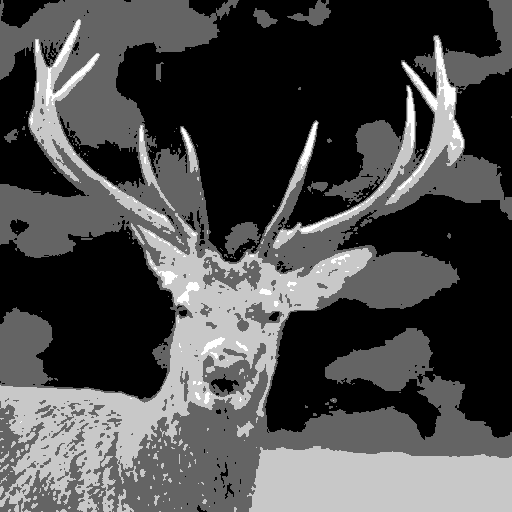
\includegraphics[scale=0.3]{./rendus/cerf3Seuil.png}}
\caption{cerf.pgm avec des seuils de 60 128 190}
\end{figure}

Pour le seuillage avec 3 seuils, on parcours chaque pixel et on teste sa valeur si celle-ci est inférieure au premier seuil on met à 0 (noir) ce pixel dans le tableau de l'image de sortie,sinon si il est inférieur au 2e seuil on le met à 128 (gris) sinon à 255 (blanc).

\newpage
\section{Profil d'une image pgm}

\begin{figure}[h]
\centerline{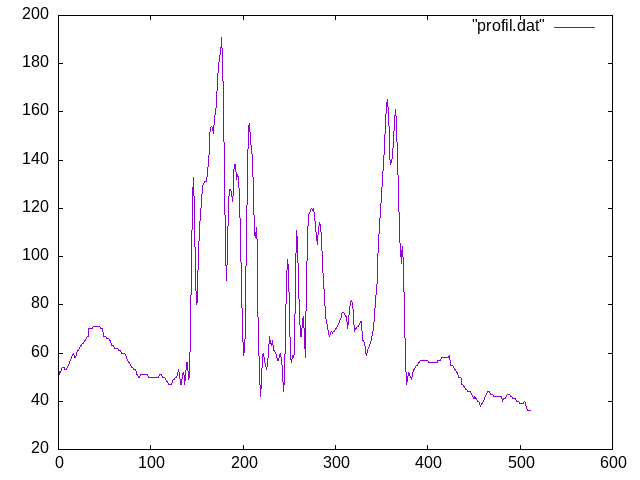
\includegraphics[scale=0.5]{./rendus/profilpgmcerf.png}}
\caption{profil de cerf.pgm colonne 250}
\end{figure}

Pour faire le profil d'une ligne ou d'une colonne, il faut pour la ligne ou la colonne donnée parcourir toutes les valeurs en faisant varier notre indice de boucle pour récupérer toutes les valeurs de cette colonne ou de cette ligne, puis faire un graphe avec gnuplot.

\newpage
\section{Histogramme d'une image pgm}

\begin{figure}[h]
\centerline{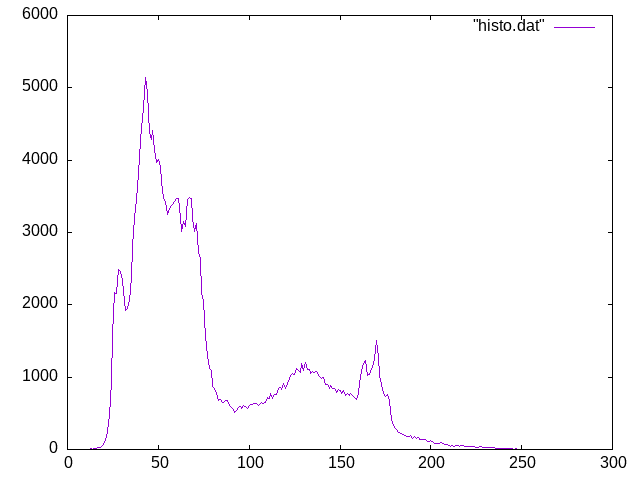
\includegraphics[scale=0.5]{./rendus/histopgmcerf.png}}
\caption{histogramme cerf.pgm}
\end{figure}

Pour faire l'histogramme d'une image pgm on va créer un tableau de 256 cases, chaque case i est le nombre d'occurences de la couleur i, puis on parcours chaque pixel de notre image et on incrémente de 1 dans la vaeur de la case i lorsqu'on tombe sur la couleur i et en faire un graphe avec gnuplot.

\section{Histogramme d'une image ppm}

\begin{figure}[h]
\centerline{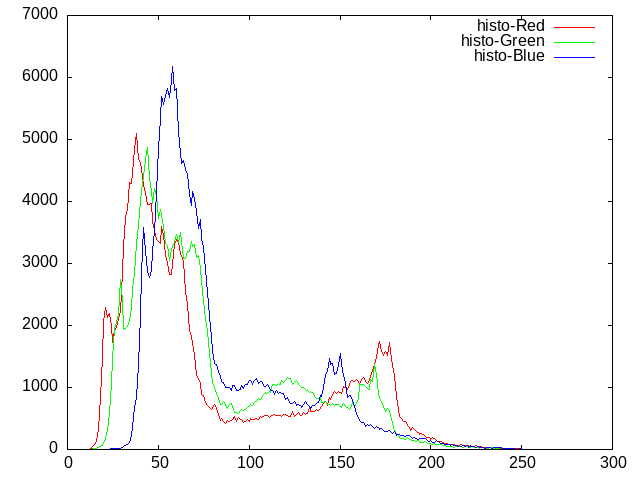
\includegraphics[scale=0.5]{./rendus/histoppmcerf.png}}
\caption{histogramme cerf.ppm}
\end{figure}

Pour faire l'histogramme d'une image couleur (RGB) on fait pareil que pour l'histogramme en pgm sauf qu'il y a maintenant 3 tableaux un pour le rouge, un autre pour le vert et un autre pour le bleu. On obtient donc 3 graphes. Il ne faut pas oublier d'incrémenter de 3 en 3 car la case i est le rouge le i+1 le vert et le i+2 le bleu pour la avoir le prochain pixel on doit donc faire incrémenter de 3.

\newpage
\section{Seuillage d'une image ppm}

\begin{figure}[h]
\centerline{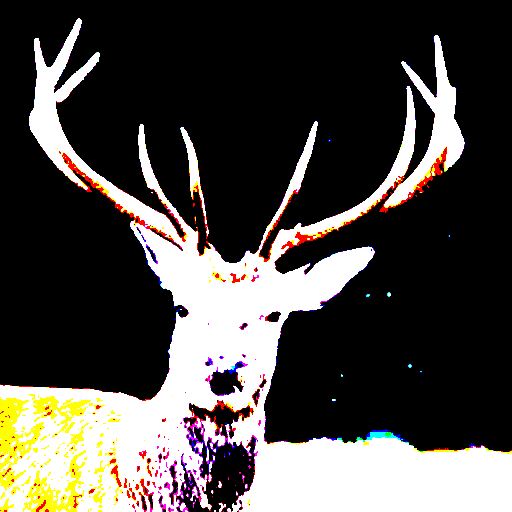
\includegraphics[scale=0.6]{./rendus/cerfSeuilppm.png}}
\caption{cerf.ppm avec des seuils de 100 (Red) 100 (Green) 100 (Blue)}
\end{figure}

Pour le seuillage d'une image ppm c'est la même chose que sur un seuillage en nuance de gris sauf que on fait ça pour les 3 composantes (Rouge, vert et bleu).

\newpage
\section{Seuillage automatique d'une image pgm}

\begin{figure}[h]
\centerline{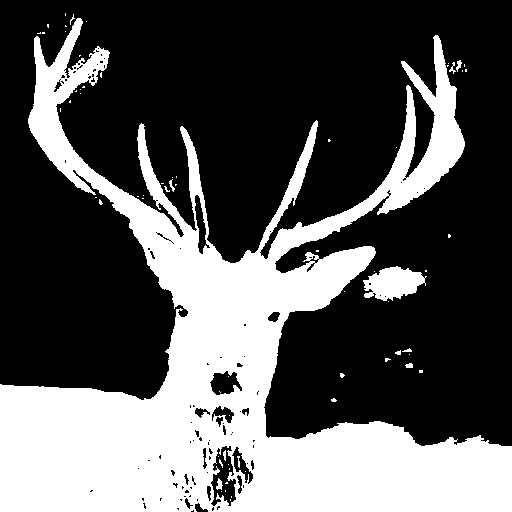
\includegraphics[scale=0.6]{./rendus/cerfSeuilauto.png}}
\caption{cerf.pgm avec un seuil automatique en utilisant la moyenne}
\end{figure}

Pour réaliser cette image seuillée on fait la moyenne des couleurs de pixel en additionnant le produit de chaque couleur et de son occurence, puis on divise par le nombre de pixels.
On remarque que le seuil automatique avec la moyenne différencie mieux le fond du cerf comparé au seuil à 128.


\end{document}